% !TEX encoding = UTF-8 Unicode

\documentclass{standalone}

% packages
\usepackage{float}
\usepackage{tabu}
\usepackage{booktabs}
\usepackage{graphicx}
\usepackage{caption}
\usepackage[export]{adjustbox}
\usepackage[utf8]{inputenc}
%\usepackage[active,pdftex,tightpage]{preview}
\usepackage{newtxtext,newtxmath}
\usepackage[percent]{overpic}

\begin{document}

%\sf
\scriptsize
\centering 

%Shallow overland water depth $(m)$ simulated by SIMWE for a $10 min$ event with $50~mm~hr^{-1}$}

\begin{tabular}{m{0.5\textwidth} m{0.5\textwidth}}

% simwe depth
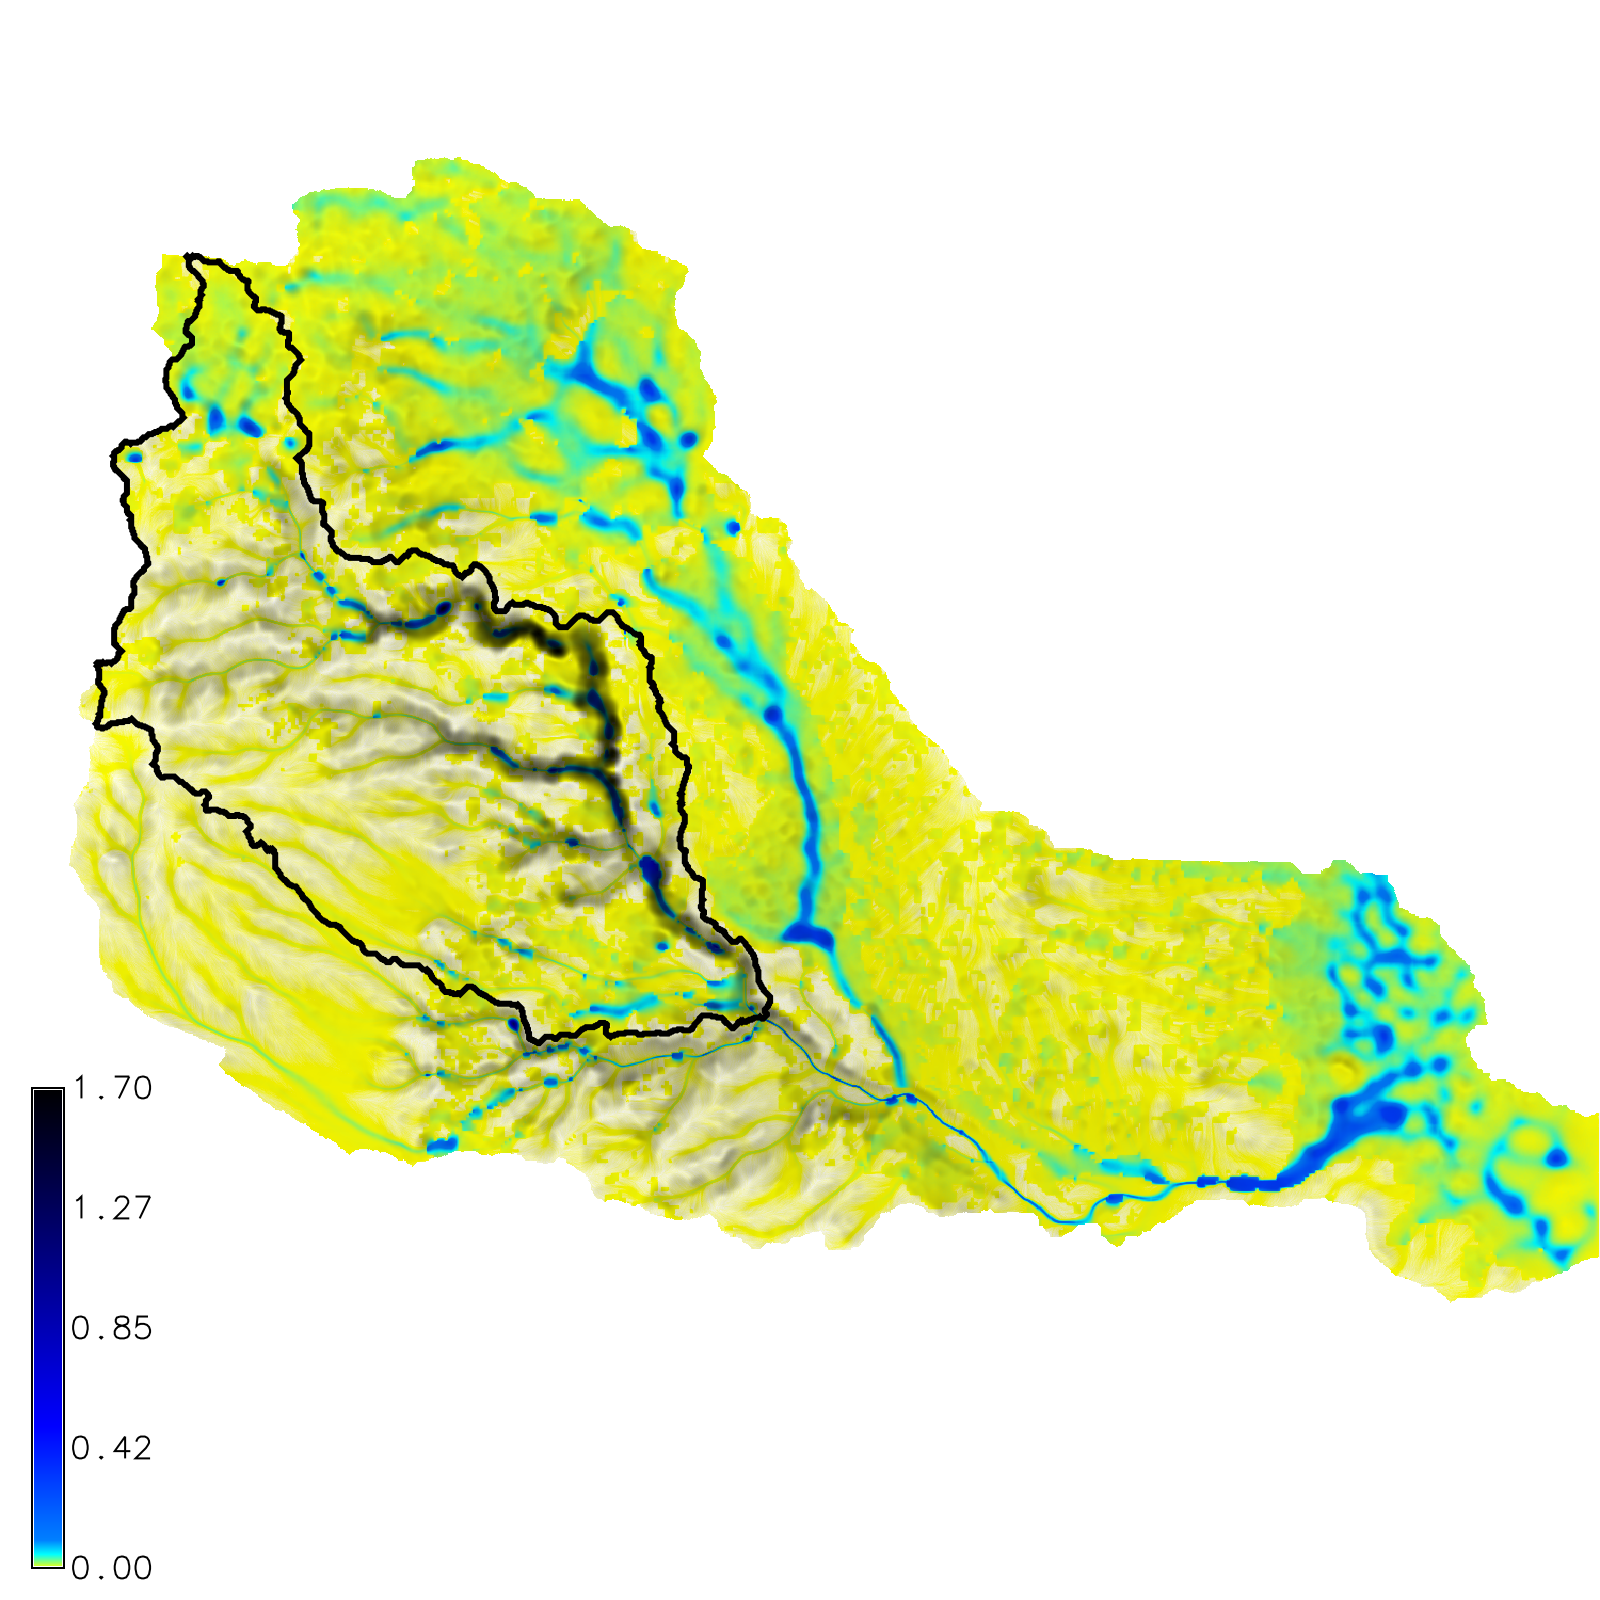
\includegraphics[height=50mm]{../../images/sample_data/depth_subwatersheds.png}&
% rusle flowacc
\begin{overpic}[height=50mm]{../../images/sample_data/flowacc_subwatersheds.png}
\put(-26,0){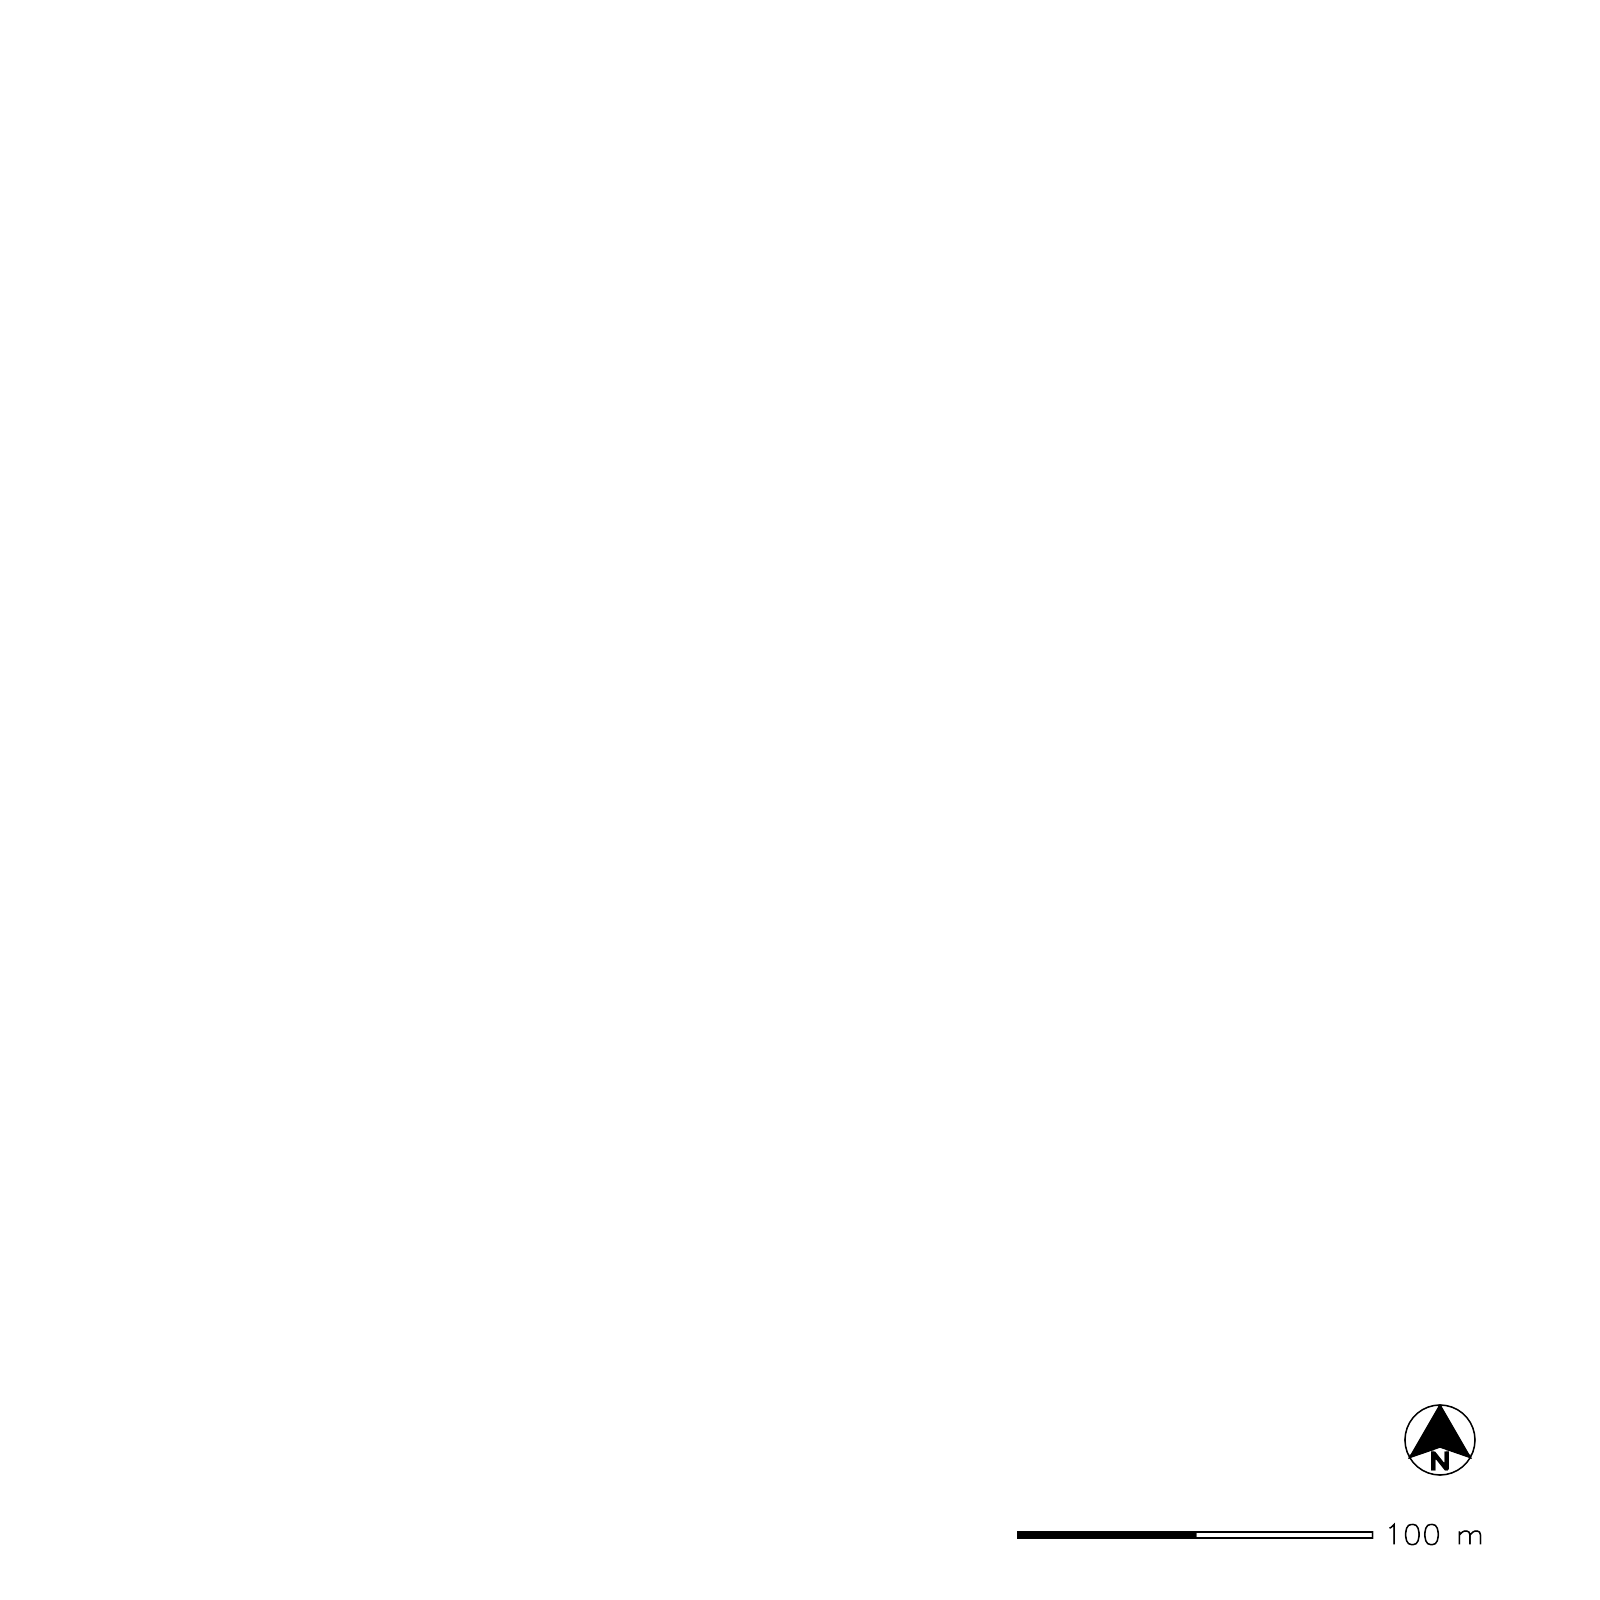
\includegraphics[height=100mm,center]{../../images/sample_data/map_elements.png}}  
\end{overpic}\\
% simwe depth caption
\multicolumn{1}{c}{a. Water depth [m] simulated by SIMWE in subwatershed}&
% rusle flow acc caption
\multicolumn{1}{c}{d. Flow accumulation for RUSLE3D in subwatershed}\\
\\
%simwe flux
\multicolumn{1}{c}{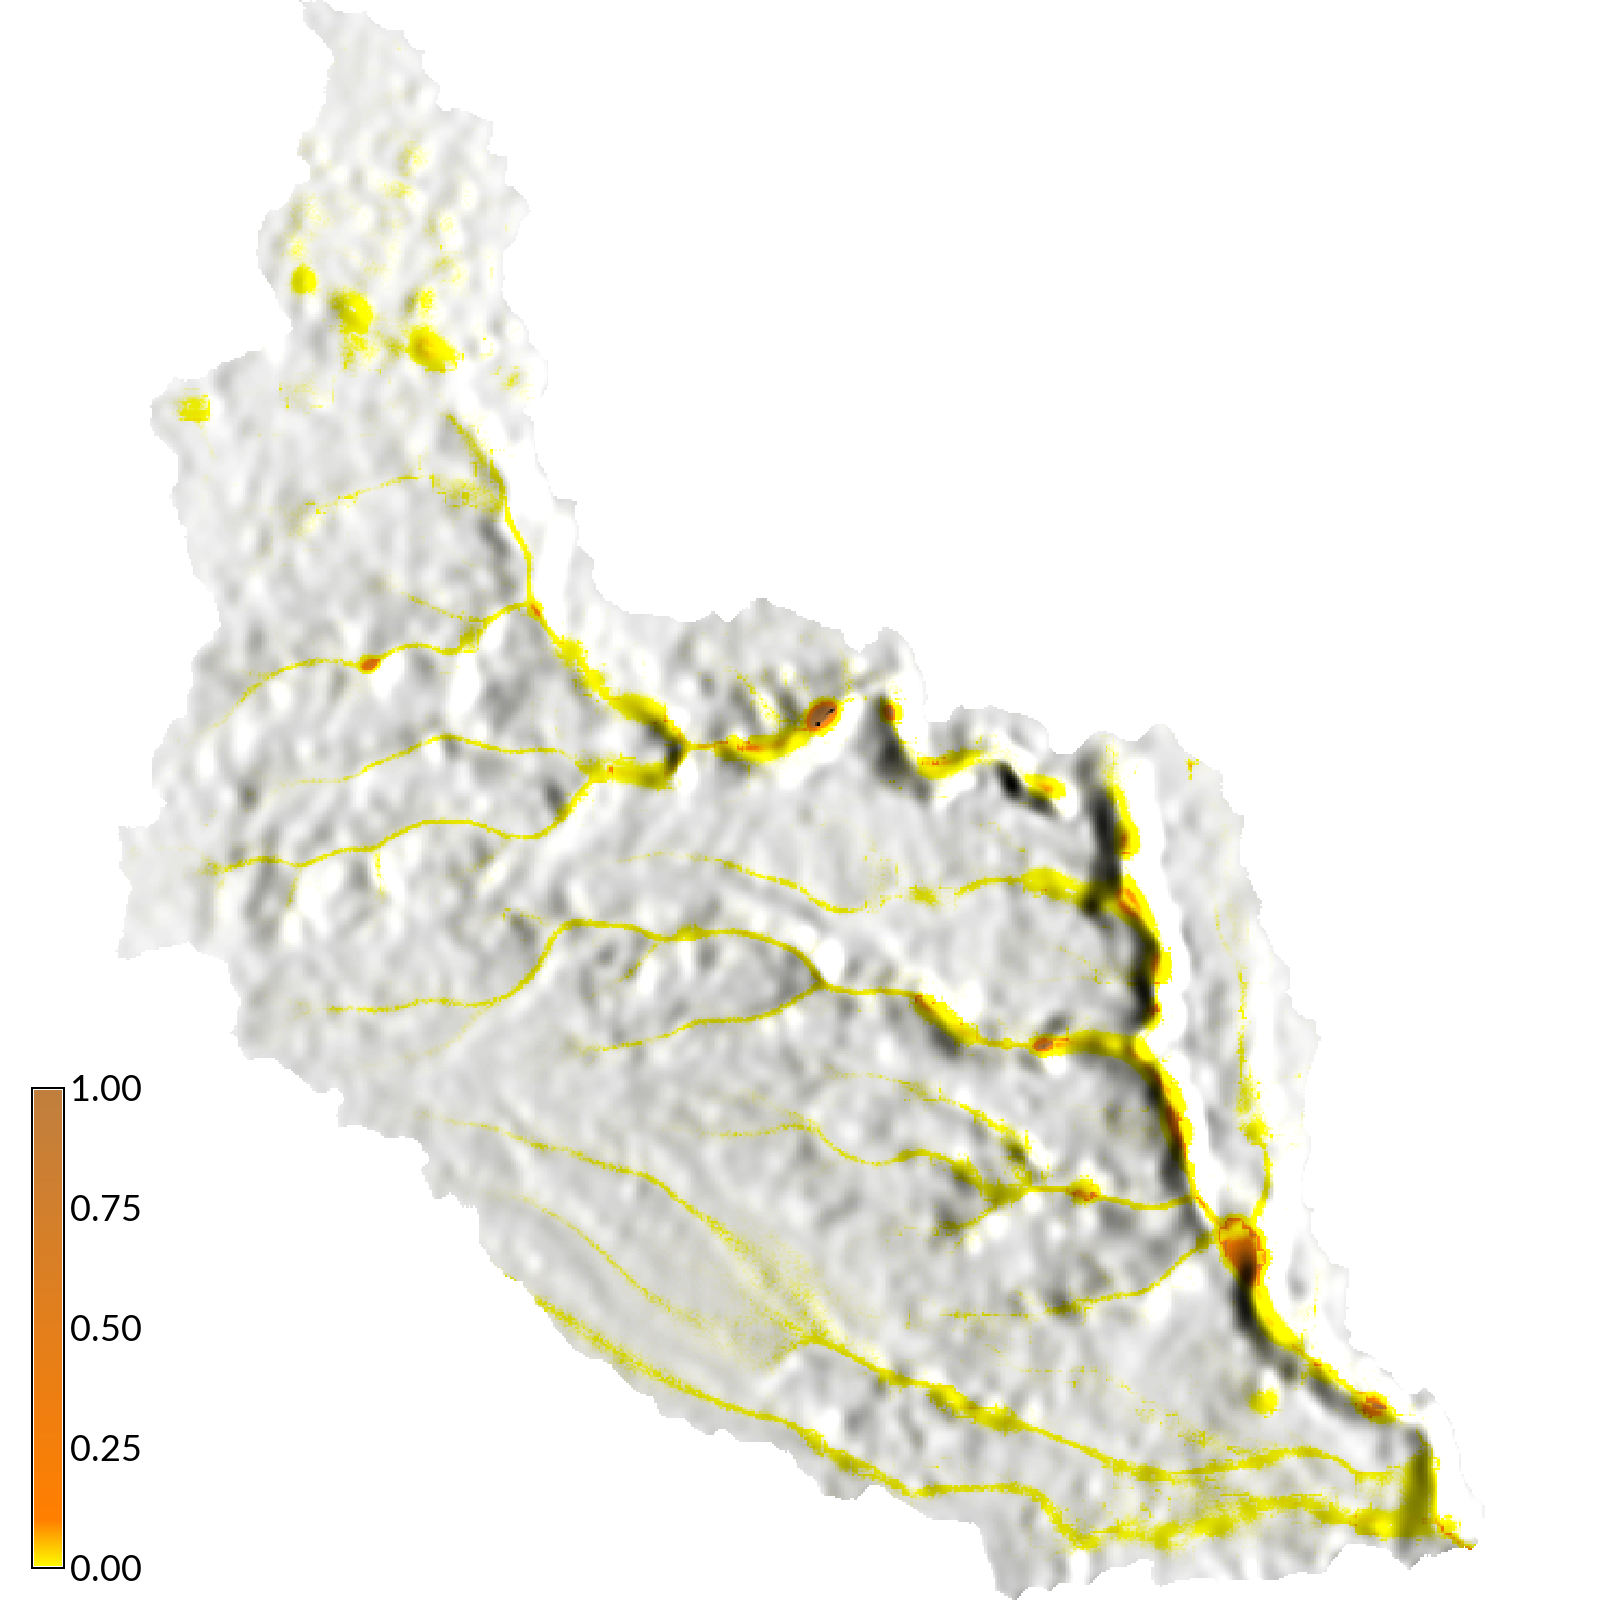
\includegraphics[height=50mm]{../../images/sample_data_detail/sediment_flux_2016.png}}&
% rusle lsfactor
\multicolumn{1}{c}{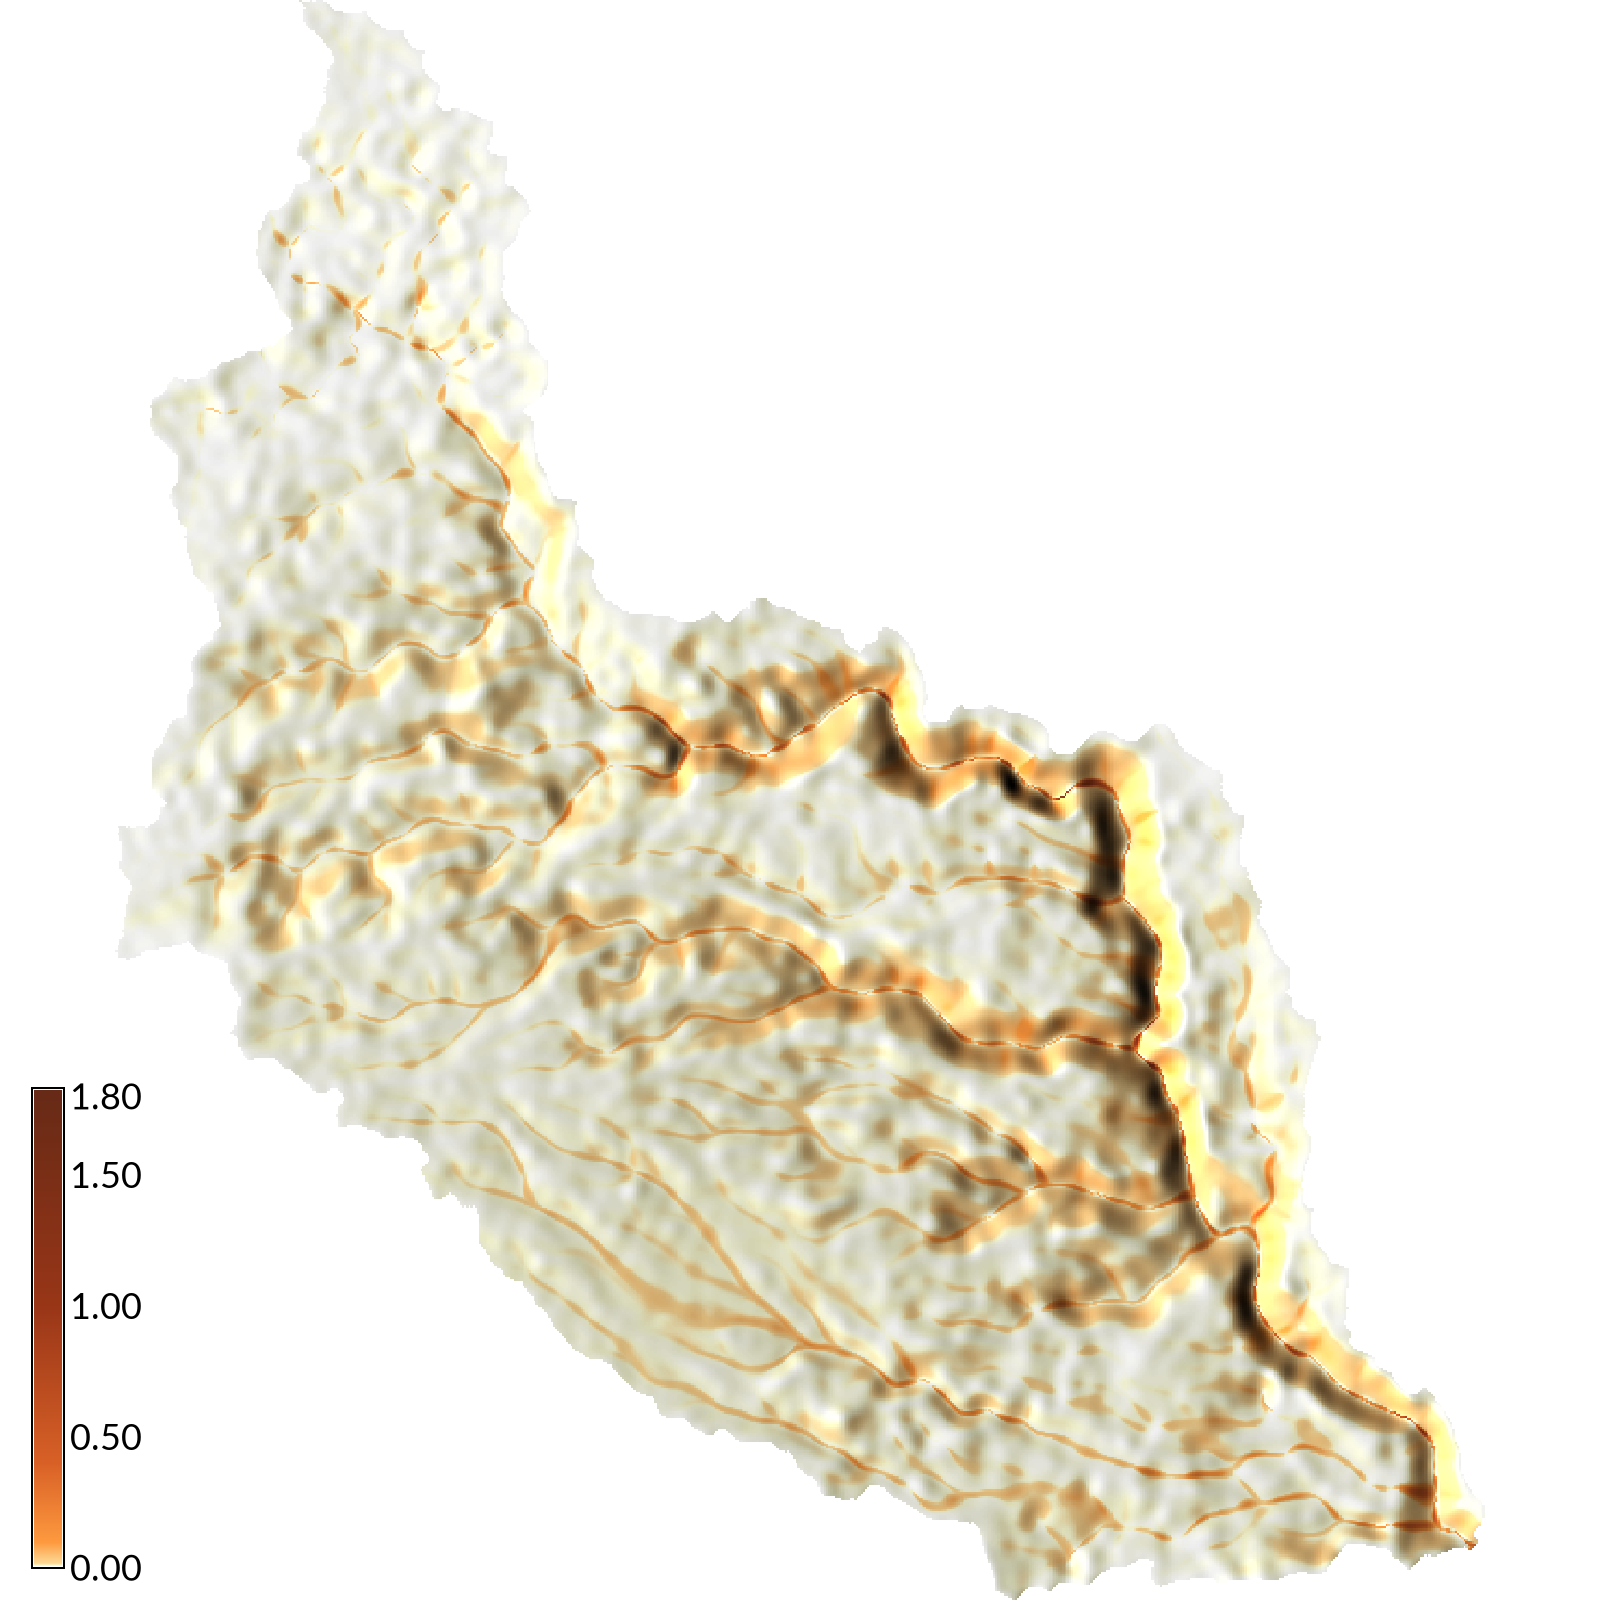
\includegraphics[height=50mm]{../../images/sample_data_detail/ls_factor.png}}\\
% simwe flux caption
\multicolumn{1}{c}{b. Sediment flux [kg~m$^{-1}$~s$^{-1}$] simulated by SIMWE}&
% rusle lsfactor caption
\multicolumn{1}{c}{e. LS3D topographic factor for RUSLE3D}\\
\multicolumn{1}{c}{in drainage area 1}
& \multicolumn{1}{c}{in drainage area 1}\\
\\
% simwe erdep
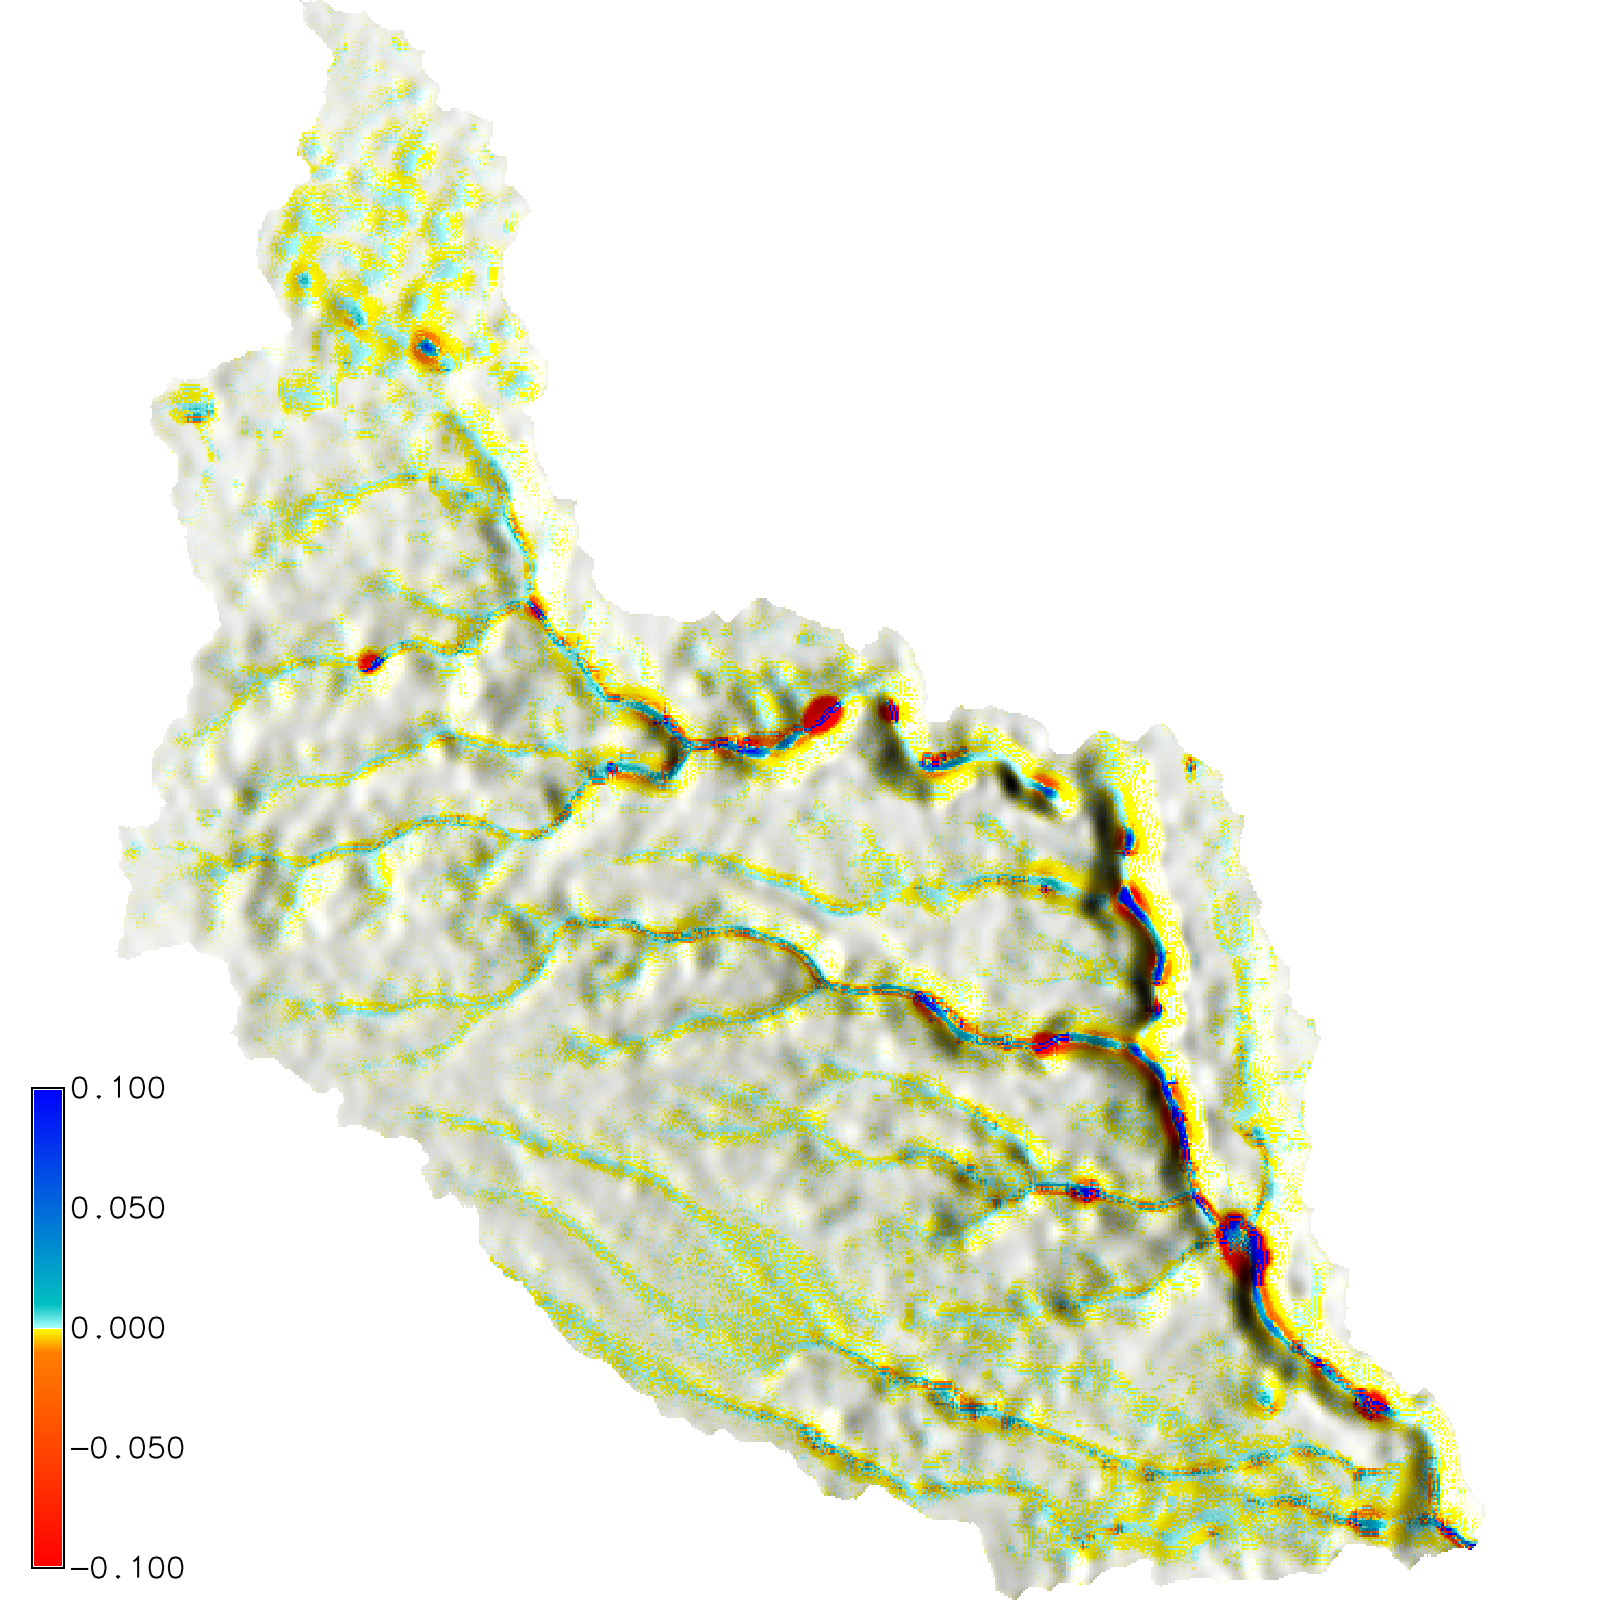
\includegraphics[height=50mm,center]{../../images/sample_data_detail/erosion_deposition_2016.png}&
% rusle sedflow
\begin{overpic}[height=50mm,center]{../../images/sample_data_detail/sediment_flow_2016.png}
\put(-22,-12){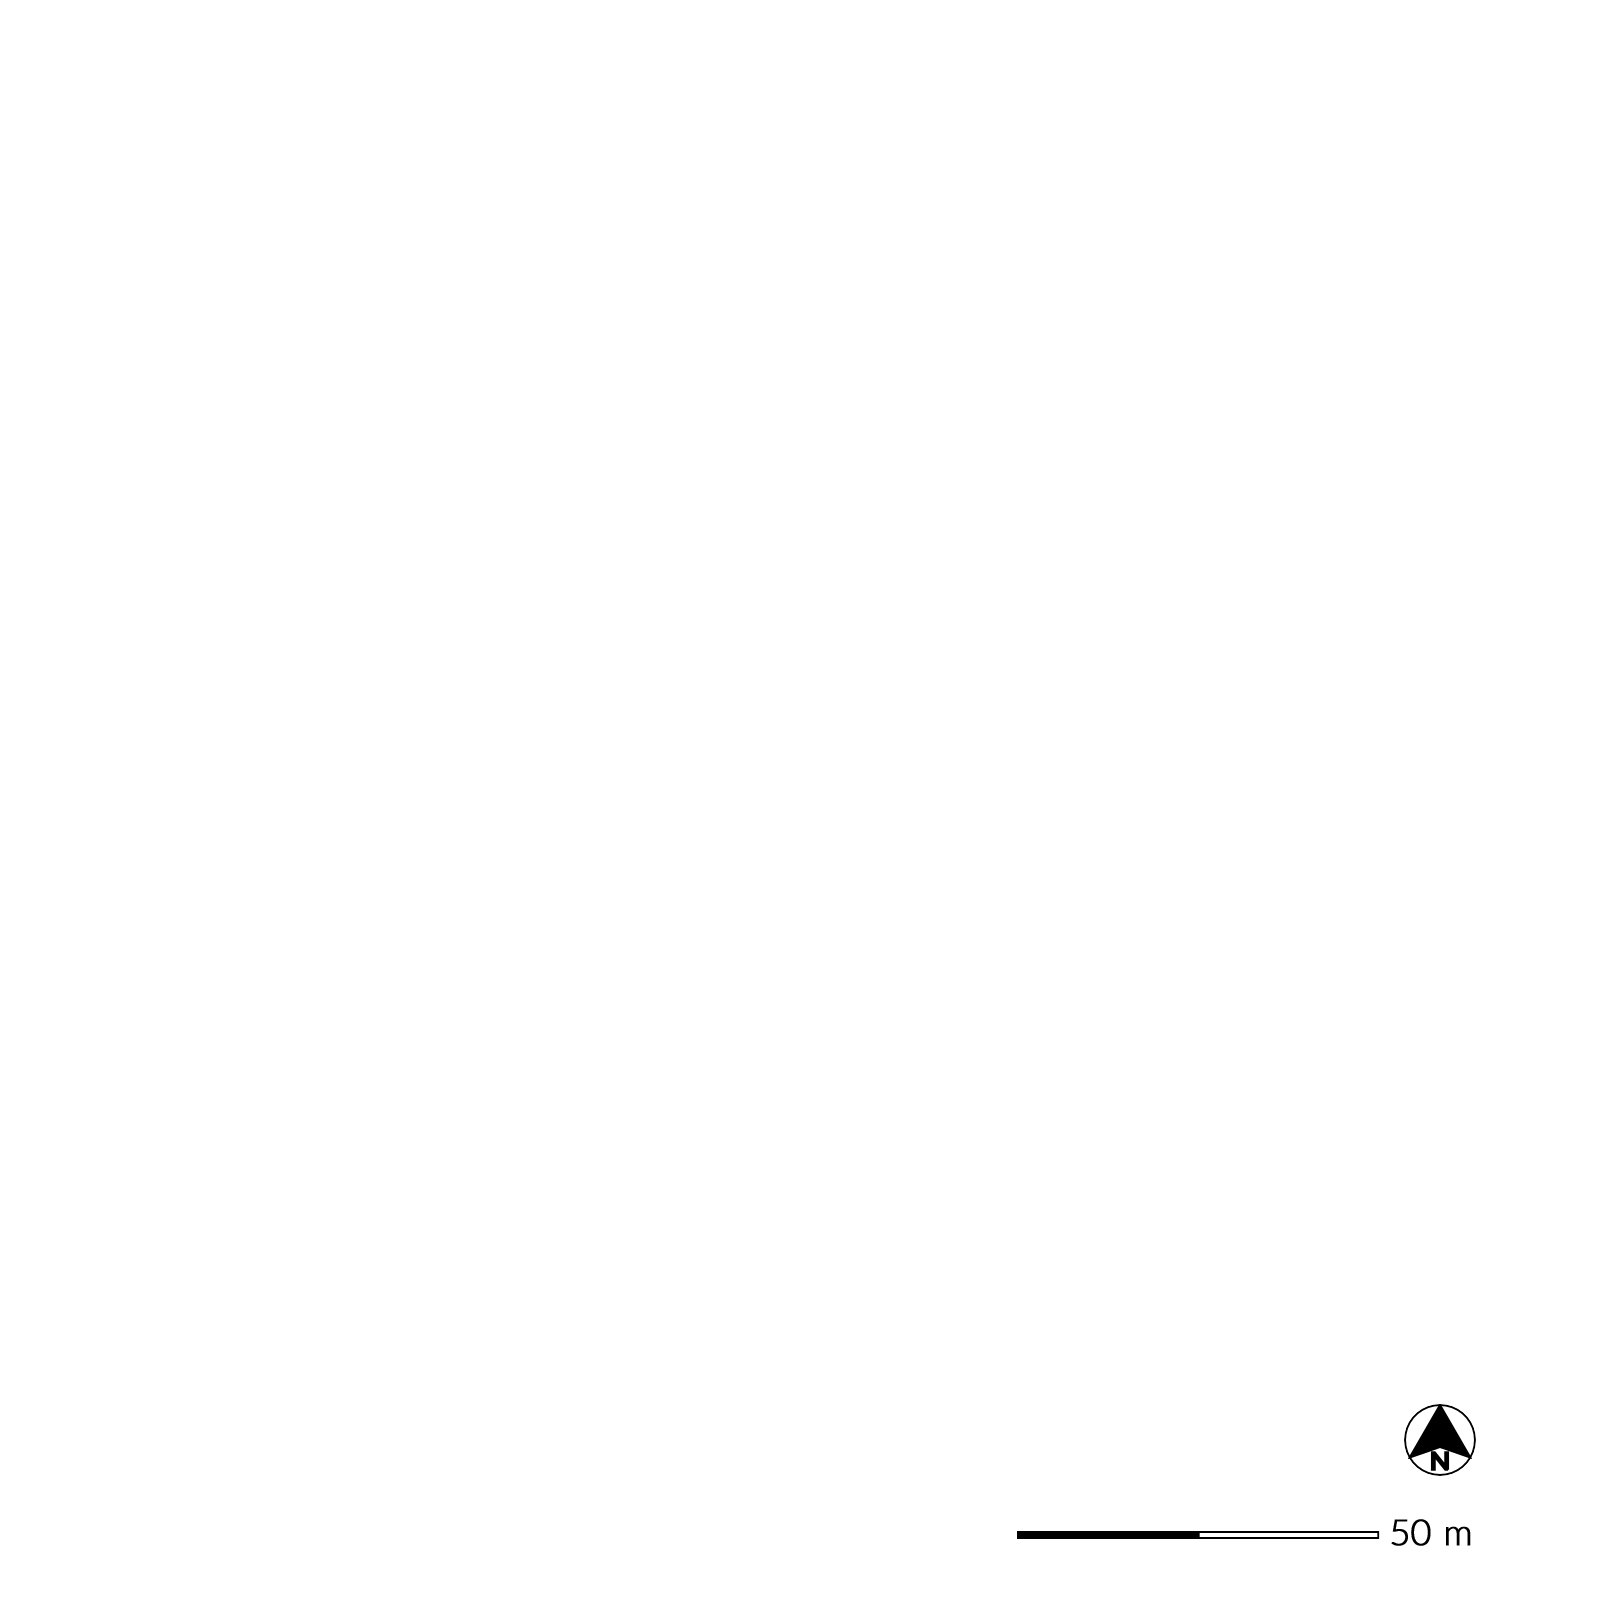
\includegraphics[height=100mm,center]{../../images/sample_data/map_elements_detail.png}}  
\end{overpic}\\
\\
\\
% simwe erdep caption
\multicolumn{1}{c}{c. Erosion and deposition [kg~m$^{-2}$~s$^{-1}$] simulated by SIMWE}&
% rusle sedflow caption
\multicolumn{1}{c}{f. Sediment flow with spatially variable landcover}\\
\multicolumn{1}{c}{in drainage area 1}
& \multicolumn{1}{c}{modeled by RUSLE3D [kg~m$^{-2}$~s$^{-1}$] in drainage area 1}\\
%
\end{tabular}

\end{document}
